\section{Explainability} \label{sec:explainability}
\cite{Doran2018}, based on a frequency analysis of explanation terms within documents from relevant research communities, highlight how different circles have different approaches to the concept of explainability and how, even within the same group, terms are used interchangeably.
In particular, they note the overloading of the notion of \enquote{explainability} with that of \enquote{interpretation}; a concept that is often defined within the xAI community as necessary for, but distinct from, explainability.
The use of \enquote{interpretable} as signifying the property belonging to a system whose inner workings are accessible can be found, for example, in the recent paper by \cite{gilpin2018explaining}.
In other recent works the two terms are conflated, for example by \cite{mittelstadt2019explaining}, \cite{guidotti2018survey} and in the influential work by \cite{doshi2017towards}.
This seems to prove the point that \cite{Lipton2016} makes in the widely-cited paper \enquote{The Mythos of Model Interpretability}, that \enquote{the task of interpretation appears underspecified. Papers provide diverse and sometimes non-overlapping motivations for interpretability, and offer myriad notions of what attributes render models interpretable.}

Most works, even those that blend the notions of interpretability and explainability, seem to agree on the end-goal that implementing such a concept should have; that is, to \enquote{summarize the reasons for neural network behavior, gain the trust of users, or produce insights about the causes of their decisions} (\cite{gilpin2018explaining}) by being able to \enquote{explain or to present in understandable terms to a human} (\cite{doshi2017towards}).
Where the consensus diverges, in defining what constitutes an explanation and the desiderata that it may have.
\cite{mittelstadt2019explaining} identify, within the literature, two broad classes of interpretability/explainability: \textit{transparency} (also called \textit{ante-hoc} explainablility) and \textit{post-hoc} interpretability.
The former type deals with the internal workings of a system while the latter applies to its external behaviour.
\cite{Lipton2016} identifies three explanations that can make a model transparent: a mechanistic understanding of the workings of the system in its entirety, of the individual components or of the algorithm.
A system may be made post-hoc interpretable by way of, among others, natural language explanations, visualisations or interactive interfaces.
These methods often do not precisely clarify the exact working of a model, but \enquote{they may nonetheless confer useful information for practitioners and end-users of machine learning.}
\cite{Biran2017} notes how the transparent or \textit{white-box} paradigm was sufficient for classic rule-based models but - with the advent of contemporary machine learning models - is no longer useful.
They argue that it is nowadays unreasonable to expect that any domain expert be able to understand a prediction if they are not also a machine learning specialist.
To address this issue, they propose a Natural Language Generation system; that is, a post-hoc explanation in \cite{Lipton2016}'s categorisation.

A widely-recognised feeling, tightly connected with the already recognised lack of shared working definitions, seems to be that researches of explainable AI are ignoring the enormous corpus of existing models in philosophy, psychology, cognitive and social sciences and human-computer interaction.
This feeling of disconnect is echoed by \cite{gilpin2018explaining} who points out how philosophical texts have long debated what constitutes an explanation, by \cite{mittelstadt2019explaining} who explicitly says how \enquote{many different people, be they lawyers, regulators, machine learning specialists, philosophers, or futurologists, are all prepared to agree on the importance of explainable AI [...] very few stop to check what they are agreeing to, and to find out what explainable AI means to other people involved in the discussion}
The fact that explainable AI researchers seem to be intent on \enquote{reinventing the wheel} is stated most strongly by \cite{miller2018explanation}, whose paper \enquote{Explanation in Artificial Intelligence: Insights from the Social Sciences} is based on the premiss that \enquote{most of the research and practice in this area seems to use the researchers' intuitions of what constitutes a `good' explanation} and argues for the adoption of the existing research in the social sciences.
The author's views are well summarised by the position xAI is set to occupy in Fig. \ref{fig:xai-position}.
The feeling is that explainable AI researchers are terming their methods \enquote{explanation} based on purely personal views and are thus building explanations that only work for themselves; in other words, \enquote{the inmates are running the asylum} (\cite{Miller2017}).
The following quote by \cite{guidotti2018survey}, in my view, perfectly sums up the state of the research in the field: \enquote{It is evident that the research activity in this field completely ignored the importance of studying a general and standard formalism for defining an explanation, identifying which are the properties that an explanation should guarantee, e.g., soundness, completeness, compactness and comprehensibility. Concerning this last property, there is no work that seriously addresses the problem of quantifying the grade of comprehensibility of an explanation for humans, although it is of fundamental importance.}

\begin{figure}[htbp]
\centerline{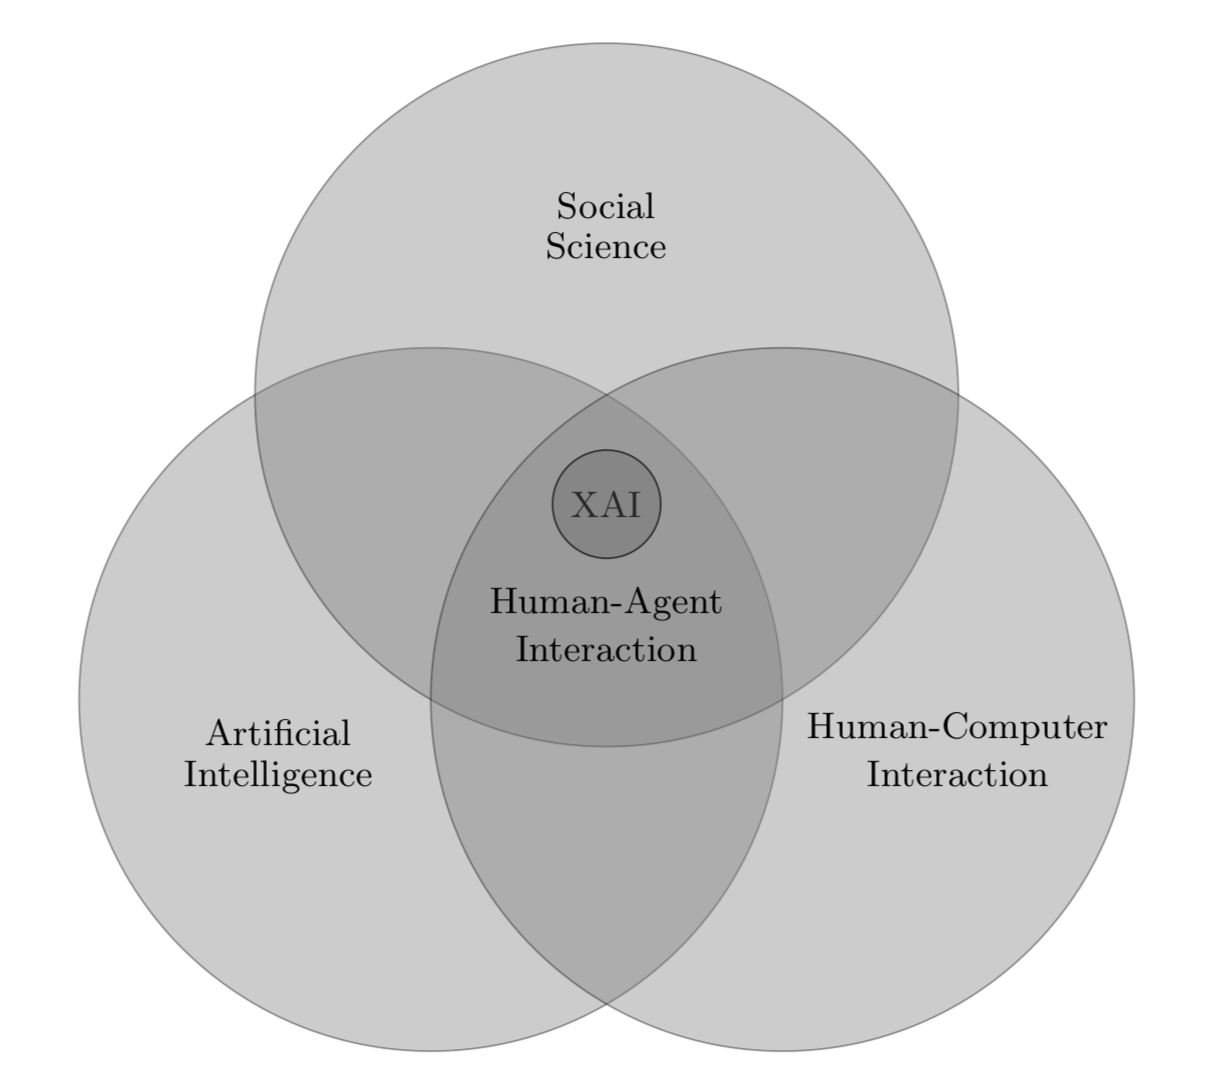
\includegraphics[width=\columnwidth/2]{literature-review/images/xai-position}}
\caption{\cite{miller2018explanation}}
\label{fig:xai-position}
\end{figure}

To remedy to this state of affairs, there have been a number of works, such as \cite{doshi2017towards}'s, that attempted to define what an explanation means and to reach consensus on it.
The most compelling attempt is in the paper \enquote{What Does Explainable AI Really Mean? A New Conceptualization of Perspectives} where \cite{Doran2018} try to synthesise the current state of affairs into a taxonomy of models:
\begin{itemize}
  \item Opaque systems: systems where the mapping from inputs to outputs is entirely inaccessible to the user.
  \item Interpretable systems: systems whose inner workings are inspectable from the outside, but that makes no effort to clarify them.
  \item Comprehensible systems: systems that emit extra information together with their output.
  \item Explainable systems: systems that explicitly output a human-understandable line of reasoning i.e., an explanation.
\end{itemize}
It is recognised, thus implicitly accepting the view that xAI should learn from the social sciences, that comprensibility depends not only on the system's characteristics, but also on the user's ability and knowledge.
Comprensibility and Interpretability are seen as separate concepts as comprehension requires transparency but interpretation does not, as the user may reason over only the emitted extra symbols.
This notion of comprensibility is expanded into that of \textit{real} explainability, that is based on a notion of \enquote{ability to formulate, for the user, a line of \textit{reasoning} that explains the decision making process of a model using \textit{human-understandable features of the input data}.} (italics by the authors).

\section{Importance of Explainability} \label{sec:importance-of-explainability}
As noted by \cite{edwards2018enslaving}, \enquote{businesses and governments are increasingly deploying machine learning (ML) systems to make and support decisions that have a crucial impact on everyday life} so, as \cite{gilpin2018explaining} say, \enquote{it becomes necessary for these mechanisms to explain themselves}.
This feeling of urgency and purpose is echoed throughout the reviewed literature; it seems, that even if researchers and the field as a whole cannot agree on a definition of explainability (as discussed in Sec. \ref{sec:explainability}), there is a keen awareness on the need for models to be explainable.
This intense urge to define explainability and, at the same time, try and create models exhibiting this property, may be counterproductive as the field risks fragmenting into a series of diverging strands, as noted by \cite{abdul2018trends} and visualised in Fig. \ref{fig:xai-citation-network}.

\begin{figure}[htbp]
\centerline{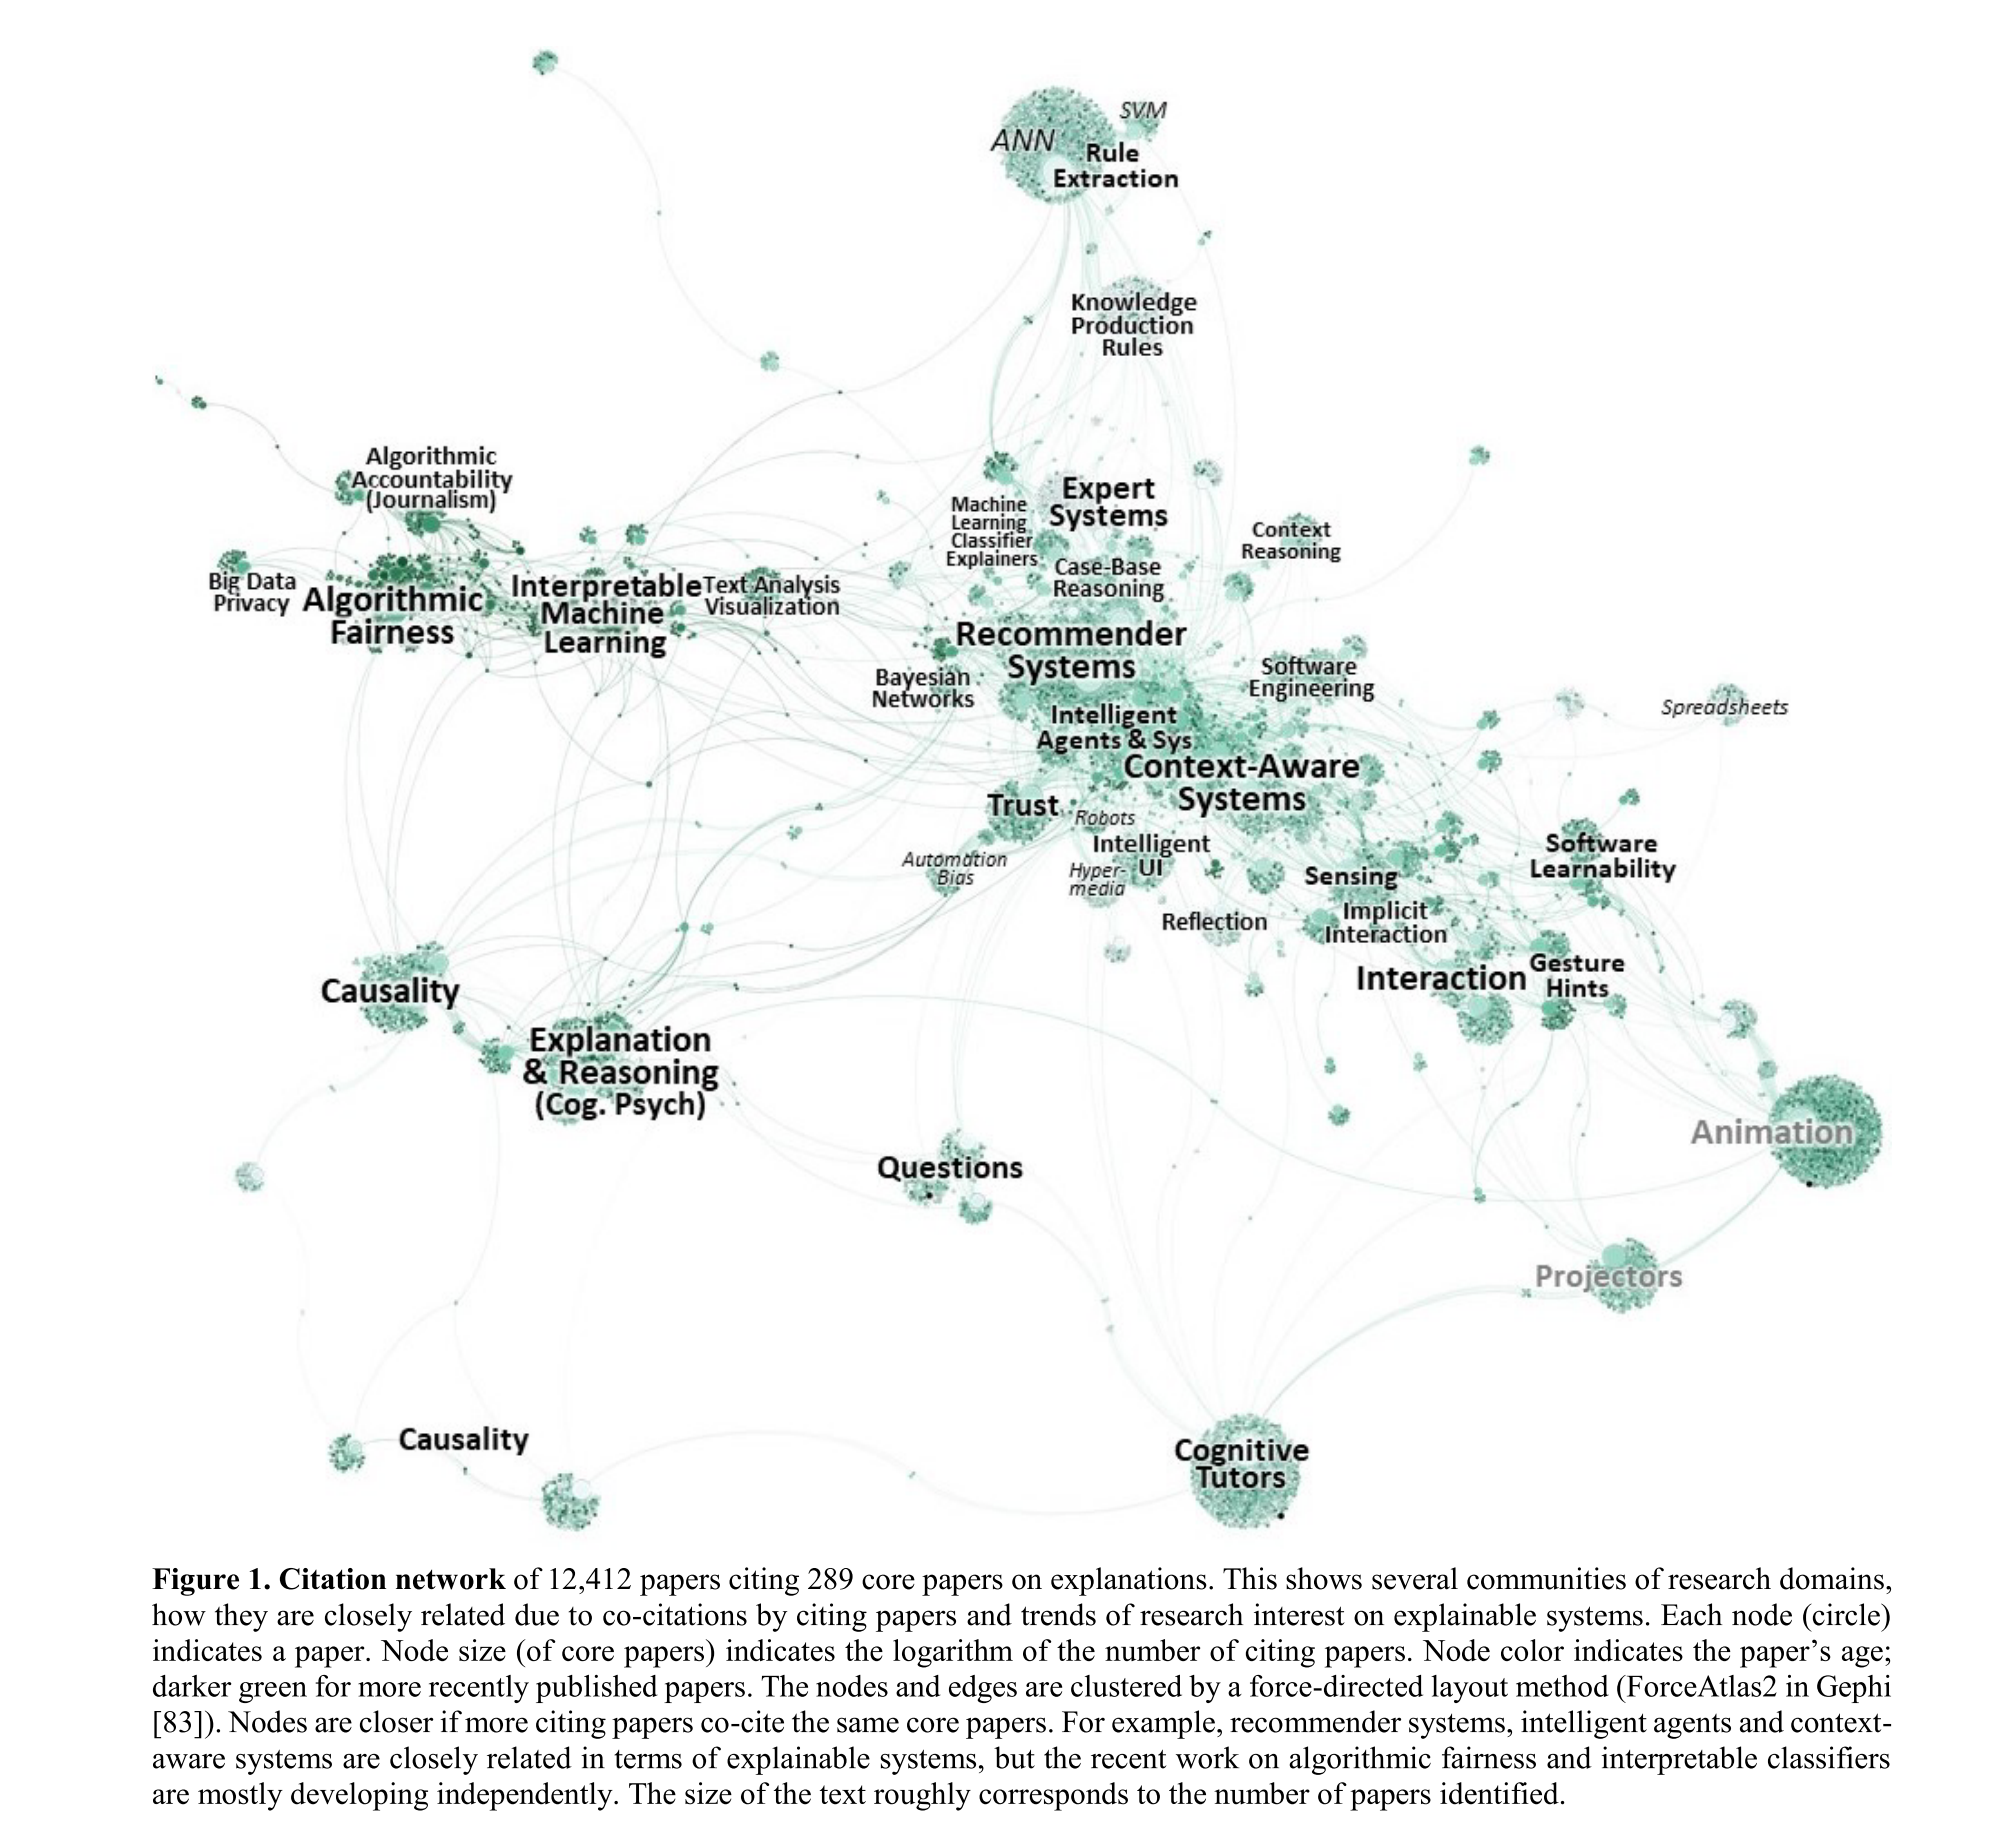
\includegraphics[width=\columnwidth]{literature-review/images/xai-citation-network}}
\caption{\cite{abdul2018trends}}
\label{fig:xai-citation-network}
\end{figure}

There are a myriad of reasons that are brought forth as a justification for the development of explainable AI, and we will review these in the following paragraphs, but it seems timely to start with one in particular: the need introduced by the European Union's broad General Data Protection Regulation (GDPR).
The GDPR was approved by the European Parliament in 2016 and came into effect in 2018.
More than one author cites an urgency to conform to this regulation (for example \cite{doshi2017towards}, \cite{gilpin2018explaining}), most likely referring to Article 22 of the regulation that, supposedly, mandates for a \enquote{right to an explanation} of algorithms.
While algorithmic explainability is undoubtedly a commendable end-goal, it may be the case that this reason, in particular, to strive for it be a false one.
\cite{edwards2018enslaving} posit that Article 22 of the GDPR actually does not contain the publicised right to an explanation but is \enquote{merely a right to stop processing unless a human is introduced to review the decision on challenge} and as the authors point out, there are, nowadays at least, very few systems without a human in the loop.
Secondly, there is no mandate for the \enquote{explanation} to be human-understandable, so the obtained result may actually be no explanation at all.
If the analysis of \cite{edwards2018enslaving} were correct, then the urgency advocated by many researchers on the grounds of conforming to the GDPR would turn out to be based on no valid reason.

A second motive brought forth for the necessity of explainability, for example by \cite{gilpin2018explaining} and \cite{abdul2018trends}, is that comprehensible models are much more likely, or even necessary, to engender users' trust.
While this may very probably be the case, no motives are given for why this should be the purpose of explainable AI and not just a desirable by-product of obtaining explainability. 

Other authors, for example, \cite{doshi2017towards} and \cite{guidotti2018survey}, frame the issue as one of moral necessity.
One need not look far to find examples of ML models displaying covert bias or making decisions we would regard as unethical; a more in-depth investigation would reveal that this was the case even before the popularisation of \enquote{black box} models as the Deep Neural Networks.
\cite{guidotti2018survey} give a reasonably comprehensive list of classic cases that show the risks of not having comprehensible AI.
The oldest of these dates back to the 1970s and 1980s and tells of a system used to screen job applicants that, even though programmed to ignore people's ethnicity, was still seen to discriminate against minorities.
In the same vein but much more recent, the American Military discovered that their computer vision system, that was developed to differentiate between enemy and friendly tanks automatically, had poor accuracy because it had learned to use the background information of the test set photos instead of the pixels representing the actual tanks.
Both these cases exemplify how an algorithm may make \enquote{wrong} inferences based on spurious or latent information that was already in the data set but that no human could have imagined being relevant.
Other failures epitomise how a model may learn our own social biases; for example, a recent Princeton study (\cite{caliskan2017semantics}) proved how models trained on web text corpora showed marked biases (towards race, gender ...) that reflected our the ones present in our own society.
Because of their findings, the authors went as far as to suggest that transparency would not be enough to uproot biases, as the very \textit{semantics} reflects biases latent in our culture. 

The driving motivation and sense of urgency present in all of the reviewed literature is quite certainly tied to the renewed interest and applicability of AI.
\cite{Preece2018} claim that the interest for explainability is naturally linked to the interest in AI itself; if this were true, then it would confirm that a need for transparency is implicit in the field itself.
This would validate the assertion made by \cite{doshi2017towards}, that the need for an explanation stems from an incompleteness in the formalisation.
\cite{Lipton2016} also acknowledges this and states that \enquote{the demand for interpretability arises when there is a mismatch between the formal objectives of supervised learning and the real world costs in a deployment setting}.
In the presence of such uncertainty, rendering the resulting model open to inspection would make the \enquote{gaps in problem formalization visible to us} and thus enable us to apply our best human judgement to evaluate them and their consequences (\cite{doshi2017towards}).

\section{Evaluation of Explainability}
As concluded in Sec. \ref{sec:importance-of-explainability}, the fact that ML models operate on incomplete assumptions makes it a necessity to have some form of evaluation of their performance.
As \cite{Lipton2016} states, \enquote{it turns out that many situations arise when our real world objectives are difficult to encode as simple real-valued functions} and this could lead to evident difficulties in optimising with respect to soft, but of paramount importance, concepts such as ethics and legality.
Being able to evaluate an automated explanation lets us \enquote{serve those objectives that we deem necessary but struggle to model formally}.

Unfortunately, the finding outlined in Sec. \ref{sec:explainability} that there is no consensus on the definition of explainability also necessarily entails that there is no agreed-upon methodology to evaluate such a property.
\cite{doshi2017towards} note as much when they comment \enquote{unfortunately, there is little consensus on what interpretability in machine learning is and how to evaluate it for benchmarking}.
This makes perfect sense because trying to evaluate something without first having defined it, is worse than trying to hit a moving target.
Once again, the feeling among many authors is that \enquote{inmates are running the asylum}.

Some authors have tried to put some order in the barrage of methods; \cite{doshi2017towards} provide one of the most compelling attempts.
 \cite{doshi2017towards} set out to outline a taxonomy, having noted a \enquote{lack of rigour} and how current interpretability approaches usually fall into two categories: interpretability in the context of an application and interpretability via a quantifiable proxy.
 The former approach assumes that \enquote{if the system is useful in either a practical application or a simplified version of it, then it must be somehow interpretable}; the latter sees researchers claim that a model class is interpretable and then present algorithms to optimise within that class.
 In their words, both classes rely on a notion of \enquote{you'll know it when you see it}.
 The taxonomy the authors lay out is shown in Fig. \ref{fig:xai-taxonomy} and borrows from methods already standard in human-computer interaction and visualisation; the guiding ideal is that \enquote{evaluation of applied work should demonstrate success in the application} and thus the best sort of evaluation is the one that involves humans the most.
 Thus, at the lowest level, they pose \enquote{Functionally-grounded Evaluations} that require no human in the loop and evaluate the quality of an explanation using some proxy measure; the advantage is the low cost, but the tradeoff is a lack of specificity.
 A proxy measure that has already been human-validated, for example a decision tree, a set of rules or a linear model (\cite{guidotti2018survey}) as regards its explainability, may be an appropriate measure for more exotic systems.
 The second level of evaluation, \enquote{Human-grounded Evaluation}, involves humans, albeit not domain expert ones; this kind of setup enables the testing of more general notions of explainability.
Finally, \enquote{Application-grounded Evaluation} is taken as the gold standard to demonstrate success in the context of an application; the authors claim that there is no better way to evaluate the quality of an explanation that having a domain expert test it in the context of a real task.
In their words, \enquote{the best way to show that the model works is to evaluate it with respect to the task}: \enquote{for example, a visualization for correcting segmentations from microscopy data would be evaluated via user studies on segmentation on the target image task; a homework-hint system is evaluated on whether the student achieves better post-test performance.  Specifically, we evaluate the quality of an explanation in the context of its end-task, such as whether it results in better identification of errors, new facts, or less discrimination}.

\begin{figure}[htbp]
\centerline{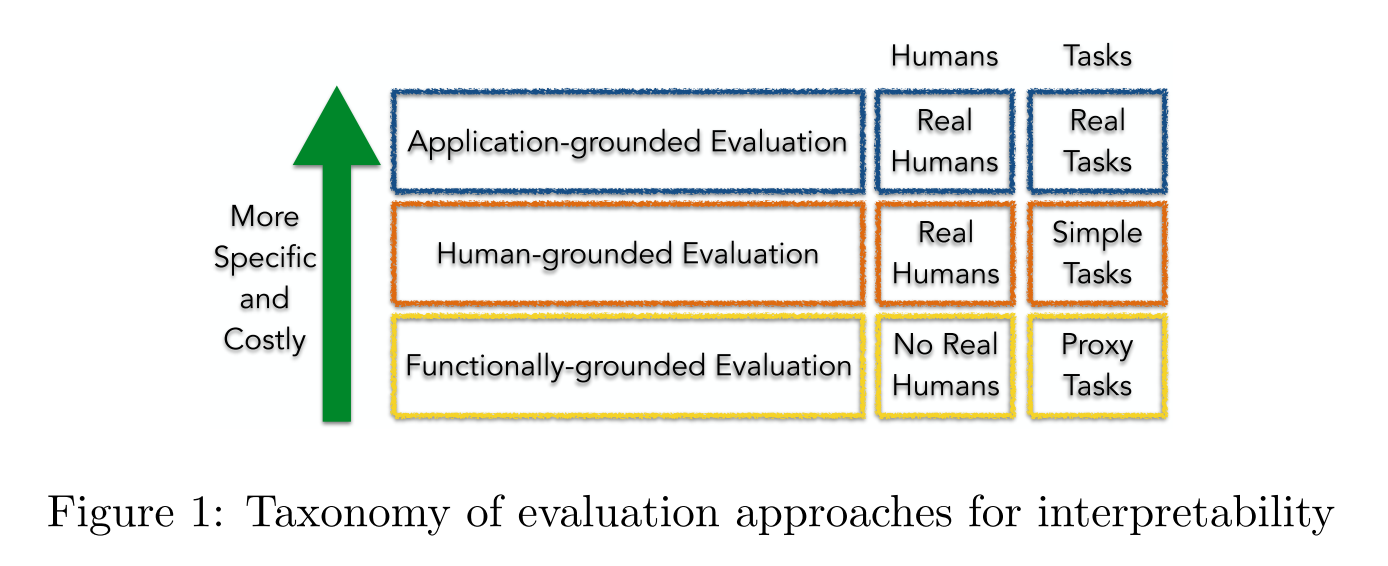
\includegraphics[width=\columnwidth]{literature-review/images/xai-taxonomy}}
\caption{\cite{doshi2017towards}}
\label{fig:xai-taxonomy}
\end{figure}

\cite{guidotti2018survey} outline a taxonomy developed along a different axis; specifically they identify: methods to explain black box models, methods to explain black box outcomes, methods to inspect black boxes and methods to design transparent boxes.
An essential factor that the authors identify is that evaluation is a graded notion, as also noted by \cite{gilpin2018explaining}: different users, with different expertise and background, may rate the quality of explanations differently.
Another point they make that is quite novel is that time should also be part of an evaluation; depending on the available time a user may prefer a more straightfoward or more elaborate explanation.
They end by noting that very few works take user expertise and the time taken to understand the proposed explanation into account.

The neglect of the human side of explanations is also lamented by \cite{abdul2018trends} who see researchers focusing on creating mathematically-explainable models at the expense of ones that are usable and practical in real-world situations.
Again, the underlying issue seems to be that xAI researchers are unaware or ignoring the sizeable corpus of research available in cognitive psychology, human-computer interfaces and philosophy.
The author sees the opportunity for HCI to bridge the gap between models and users by way of an interactive approach, as opposed to the mainstream static explanations being proposed in the literature.
An interactive explanation may take the form of a dialogue or of various visualisation techniques; the defining characteristic of such a mode is that it lets the user freely explore the system's behaviour.
\cite{guidotti2018survey}, while discussing the types of data used in ML models, lend credence to the goodness of this output modality with the statement that \enquote{other forms of data which are very common in daily human life are images and texts. They are perhaps for human brain even more easily understandable than tables}.

\cite{guidotti2018survey}, though, take the view that evaluation of model \textit{complexity} should be equated to its \textit{comprehensibility}, that is not something that often appears in the relevant literature.
Basically, the authors are advocating for the use of complexity as a proxy model for explainability, if we are framing the issue using the taxonomy proposed by \cite{doshi2017towards} (Fig. \ref{fig:xai-taxonomy}).
This may very well be a valid approach, but there is no supporting evidence for it in the paper itself.

A useful reference for how to set up an experiment falling into the class of either Human-grounded or Application-grounded Evaluation can be found in \cite{stumpf2009interacting}'s \enquote{Interacting meaningfully with machine learning systems: Three experiments} 2009 paper.
In this work the authors set up \enquote{three experiments to understand the potential for rich interactions between users and machine learning systems}; the first, and most relevant, was a think-aloud study that investigated \enquote{how machine learning systems should explain themselves to end users, and what kinds of improvement feedback end users might give to the machine learning systems}.
These studies are interesting as a blueprint for future human-centred evaluations, of the type whose absence is being lamented by many authors.

\cite{mittelstadt2019explaining} summarise the existing critiques to offer a clear and direct evaluation of the field of Explainable AI as a whole, when they state that \enquote{no matter the approach taken in xAI, reflexivity \textit{[taking account of itself or of the effect of the personality or presence of the researcher on what is being investigated], my note} is needed to ensure the community actually works towards its normative and practical goals to render models holistically transparent or provide high-quality post-hoc interpretations of model behaviour. Critical questions must be repeatedly asked and answered. For example, will the methods developed make machine learning models more interpretable? More trustworthy to users? More accountable? And to whom will explanations be accessible, comprehensible, and useful? Answering such questions requires considering the methods developed in xAI in the context of prior work in fields addressing such normative and social questions. Local and approximation models may in fact resemble existing, well-known approaches to explanations in the `explanation sciences', which would provide insight}.
They then conclude by stating that \enquote{xAI generally avoids the challenges of testing and validating approximation models, or fully characterising their domain}.
From the review of the current state-of-the-art carried out in this section and Sec. \ref{sec:explainability} and \ref{sec:importance-of-explainability}, these could both be seen as entirely valid criticisms.
It really seems that the field of xAI as a whole should try and reposition itself as suggested in Fig. \ref{fig:xai-position} and not try to build methods from first principles, many of which may be outside the domain of expertise of the researchers in question.

\section{Explainability of Bayesian Networks} \label{sec:explainability-in-bayesian-networks}
Bayesian Networks have enjoyed widespread appeal as a Machine Learning method, especially inside the medical domain.
This may be because the formalism (introduced in detail in Sec. \ref{sec:bayesiannetworks}) \enquote{offers a natural way to represent the uncertainties involved in medicine when dealing
with diagnosis, treatment selection, planning, and prediction of prognosis. This is due to the fact that the influences and probabilistic interactions among variables can be described readily in a BN} (\cite{Lucas2001}); that is, even if the BN model is \textit{complete}, in the sense that every possible probabilistic statement can be computed in it, it also is easy to combine multiple variables of interest into composite questions.
Another attractive feature of BNs is their relatedness to the class of \textit{Causal Networks} that were popularised by the groundbreaking work of \cite{Pearl1988}; for all intents and purposes, a Causal Network is simply a Bayesian Network where all the relationships represent a causal effect.
Nonetheless, BNs are not considered as inherently interpretable by the literature, and thus, a series of methods were developed to address this shortcoming.
\cite{timmer2015explaining} note this in the introduction to their paper by stating that \enquote{for non-statistical experts, however, Bayesian networks may be hard to interpret. Especially since the inner workings of Bayesian networks are complicated they may appear as black box models}, \enquote{the interpretation of BNs is a difficult task, especially for domain experts who are not trained in probabilistic reasoning}.

The best overview of the state of explainability in BNs is given by \cite{lacave2002review} in the paper \enquote{A review of explanation methods for Bayesian networks}; here the authors identify various classification criteria for an explanation given by a BN:
\begin{itemize}
  \item \textit{description} vs. \textit{comprehension}: the former consists in displaying the data set or providing further details regarding the output, the latter attempts to guide the user in understanding the model's conclusions.
  \item \textit{micro-level} vs. \textit{macro-level}: detailed description of how a single node is affected vs. showing the main lines of reasoning.
  \item \textit{verbal} vs. \textit{graphical}: \enquote{the most direct and intuitive way of showing the information embodied in a Bayesian network is to display the corresponding graph}.
  When presenting probabilities, \cite{henrion1990qualtitative} strongly suggest that these be \enquote{linguistic probabilities} i.e., for the quantitative probabilities inherent in the model to be converted to a qualitative equivalent.
  This is validated by research showing that linguistic expressions of probability are better understood than the equivalent numerical representation. 
  Some of the many models surveyed in the paper user colours, shading and line thickness to represent the salience of links and nodes.
\end{itemize}
The authors also identify the three components of BNs that need to be explained: the knowledge base, the reasoning process and the evidence propagated.
The first of these \enquote{consists of determining which values of the unobserved variables justify the available evidence} and is, in general, done by finding the solution to the Most Probable Explanation problem (defined in Subsec. \ref{subsec:bnupdating}).
The explanation of the model is considered a static explanation (as opposed to dynamic ones, that will shortly be covered) and is simply the process of verbally or graphically displaying the information already present in the data.
The final element to explain, that is what would most commonly be called an explanation in xAI circles, is the reasoning behind the model's outputs; a system may accomplish this by providing a justification for its outputs, for the results it did not give or via hypothetical reasoning.
The first of these is maybe the most important, because it is paramount for any system, not just a BN, to be able to explain the reasons behind its outputs; returning to the medical setting, it was seen that physicians, in particular, are very reluctant to accept the advice of a machine if they can not understand how it was obtained.
A BN, unlike other ML systems, can also innately exhibit evidence for why it did not provide the output expected by the user and can also reason \textit{counterfactually} i.e. provide alternative outputs.
These last two capabilities are particularly important, from an explainability perspective, in light of \cite{miller2018explanation}'s findings regarding the nature of explanations.

\cite{miller2018explanation}'s paper \enquote{Explanation in Artificial Intelligence: Insights from the Social Sciences} investigates what constitutes an explanation from a psychological perspective; the conclusions are that explanations possess four primary characteristics:
\begin{itemize}
  \item explanations are \textit{contrastive}; that is people do not ask why an event happened by why another event did not happen instead.  
  A Bayesian Network, as noted in the previous paragraph, is capable of modelling counterfactuals which enables them to give contrastive reasons naturally.
  \item explanations are \textit{selected}; people expect an explanation to be selected based on some cognitive bias; they do not expect a complete recount of all causes of an event.
  A BN has the ability to combine an output from its constituent variables in a flexible manner. 
  \item to people, probabilities are not as important and not as well understood as causal relationships.
  BNs, as already mentioned, are closely related to \textit{graphical causal models}, so their explanations have the possibility of being based on causal grounds (\cite{Lipton2016}, \cite{rani2006empirical}).
  \item explanations are \textit{social}; that is they involve an \textit{explainer} and an \textit{explainee}.  
  This is recognised in the most important work on the social aspects of conversation, \cite{Hilton1990}'s \enquote{Conversational processes and causal explanation}, that supports the view that an \textit{explanation} is a \textit{conversation}. 
  A dialogue is an example of a \textit{dynamical explanation}, in the framework set out by \cite{lacave2002review}; these authors also recognise that an explanation \enquote{always means explaining something to somebody} and that thus \enquote{one of the key features of an effective explanation is the ability to address each user's specific needs and expectations, which primarily depends on the knowledge he/she has}.
  	  So \enquote{In the case of a Bayesian network, the explanation generated for a user that is familiar with the concepts of prevalence, prior/posterior odds and likelihood ratios should be very different from the explanation generated for a user who has never heard about them}.
  	  \cite{lacave2002review} again recognise that explainability is a graded notion but go further and define the concept of \textit{fixed user model}, noting that practically all explainable BN systems have made this assumption and ignored the possibility of users having varying knowledge.
  	  Though, some of the systems surveyed in the paper make a step in that direction by incorporating an \textit{importance threshold} mechanism that would let the user only display certain items; this enables these systems to display varying levels of detail without having defined a user model.
\end{itemize}

Bayesian Networks, in the taxonomy set forth by \cite{Doran2018} and discussed in Sec. \ref{sec:explainability}, would most probably fall into the class of \textit{Interpretable systems}, as do many other ML models.
Though, based on the review of the literature, it could be suggested, on quite a strong basis, that Bayesian Networks are better equipped than other Machine Learning models to provide a meaningful explanation to humans.
This could be claimed because it is quite widely believed that our brains and thus our psychology are near-optimal problem-solvers and thus approximate optimal Bayesian solutions.
A standard view in the fields of psychology and neuroscience, as noted by \cite{Bowers2012}, is that our brain processes approximate the \textit{rational player} as presented in the Dutch Book Argument (see Ch.7 of \cite{anand2009handbook}) and are thus Bayesian in nature.
It is of worth to also note that this view has recently been challenged, for example by \cite{Bowers2012}.
Even if our brains were not inherently Bayesian, the characteristics of Bayesian Networks make them more capable than other ML models in being able to generate explanations tailored to our cognitive processes and psychology, as discussed in the above bullet points.
